\documentclass[sigconf,anonymous,review]{acmart}

\setcopyright{none}
\settopmatter{printacmref=false,printccs=false,printfolios=true}
\renewcommand\footnotetextcopyrightpermission[1]{}
\acmConference[WSDM 2027]{WSDM 2027}{February 2027}{Hong Kong, China}
\pagestyle{plain}

\usepackage{amsmath}
\usepackage{booktabs}
\usepackage{enumitem}
\usepackage{graphicx}
\usepackage{mdframed}
\usepackage{multirow}
\usepackage{tabularx}
\usepackage{xcolor}
\usepackage{float}
\setlength{\emergencystretch}{1em}

\newcolumntype{Y}{>{\raggedright\arraybackslash}X}
\newcolumntype{L}[1]{>{\raggedright\arraybackslash}p{#1}}
\newcommand{\pp}{\,pp}
\newcommand{\yes}{\ding{51}}
\newcommand{\no}{\ding{55}}
\newcommand{\D}{\mathrm{D}}
\newcommand{\C}{\mathrm{C}}
\newcommand{\N}{\mathrm{N}}
\newcommand{\Q}{\mathrm{Q}}

\newenvironment{promptbox}[1]{%
  \begin{mdframed}[
    backgroundcolor=black!2,
    linecolor=black!65,
    linewidth=0.55pt,
    roundcorner=1.5mm,
    innerleftmargin=1.5mm,
    innerrightmargin=1.5mm,
    innertopmargin=1.2mm,
    innerbottommargin=1.2mm,
    nobreak=true,
    skipabove=4pt,
    skipbelow=5pt,
    frametitle={\strut #1},
    frametitlebackgroundcolor=black!72,
    frametitlefontcolor=white,
    frametitlefont=\bfseries\small,
    frametitlerule=true,
    frametitlerulecolor=black!72,
    frametitleaboveskip=1mm,
    frametitlebelowskip=1mm]
  \small
}{\end{mdframed}}

\title{Supplementary Material for DoubtBench: Does Self-Doubt Help Language Models---or Just Make Them Check?}
\author{Anonymous Authors}
\date{}

\begin{document}
\maketitle

This supplement provides the complete task inventory, exact prompt
interventions, evaluation and scoring protocol, full numerical results, and
diagnostic analyses for DoubtBench.

\tableofcontents

\section{Benchmark Construction and Contents}

\subsection{Evaluation Unit and Counting Reconciliation}

A latent task contains model-visible instructions, a hidden structured state,
an exact gold answer, a task family, a task type, a difficulty level, and the
seed used to generate it. The model receives the instructions but not the
structured state, answer function, or gold answer. For a fixed checkpoint,
each latent task is evaluated under all five prompt conditions and both task
contexts. The task identifier is therefore the unit of pairing.

Table~\ref{tab:counts} reconciles the latent-task count with the number of
model responses analyzed.

\begin{table}[H]
\centering
\small
\begin{tabular}{@{}lr@{}}
\toprule
Property & Count \\
\midrule
Task families & 8 \\
Task types & 33 \\
Independently seeded task sets & 4 \\
Tasks per set & 1,600 \\
Latent tasks & 6,400 \\
Prompt conditions & 5 \\
Task contexts & 2 \\
Responses per checkpoint and latent task & 10 \\
Evaluated checkpoints & 6 \\
Main factorial responses & 384,000 \\
Latent tasks selected for surface-form analysis & 330 \\
Additional renderings (two per selected task) & 660 \\
Responses from the additional renderings & 39,600 \\
\textbf{Total completed responses} & \textbf{423,600} \\
\bottomrule
\end{tabular}
\caption{Counting reconciliation. The canonical forms of the 330 tasks used
for surface-form analysis are already included in the main factorial. Only
the two additional renderings per task contribute new responses.}
\label{tab:counts}
\end{table}

The main factorial contains $6{,}400$ latent tasks evaluated under five prompt
conditions, two task contexts, and six checkpoints, yielding
$6{,}400\times5\times2\times6=384{,}000$ responses. For the surface-form
analysis, 330 of those latent tasks were each rendered in two additional,
answer-preserving forms, producing 660 new rendered task instances. Evaluating
the added renderings under the same five prompt conditions, two task contexts,
and six checkpoints contributes
$660\times5\times2\times6=39{,}600$ additional responses. The canonical forms
of those 330 tasks are already counted in the main factorial and are not
counted again. The four task sets contain independently generated instances
from the same 33 task types. The surface-form analysis uses 330 tasks from one
of these sets.

Each task set contains 200 tasks from every family. Within each family, 80
tasks are easy, 80 are medium, and 40 are hard. Task types are allocated as
evenly as possible within a family. Across all four task sets, each family
therefore contributes 800 tasks with a 40/40/20 difficulty distribution.

\subsection{Complete Task-Type Inventory}

Table~\ref{tab:inventory} states the operation and answer representation for
all 33 task types. The family names describe operational demands in these
program-generated tasks; they do not assert equivalence to human clinical or
psychometric constructs.

\begin{table*}[!t]
\centering
\fontsize{7.0}{7.8}\selectfont
\setlength{\tabcolsep}{3.2pt}
\begin{tabularx}{\textwidth}{@{}L{2.55cm}L{2.7cm}YL{1.7cm}@{}}
\toprule
Family & Task type & Required operation & Answer representation \\
\midrule
\multirow{4}{2.55cm}{Working memory and updating}
& List updates & Apply ordered append, replacement, removal, and reversal operations & Ordered list \\
& Key-value updates & Apply assignments and swaps to labeled values & Key-value list \\
& Running counter & Update a numerical state while ignoring marked distractors & Integer \\
& Stack operations & Apply ordered push and pop operations & Ordered list \\
\addlinespace
\multirow{5}{2.55cm}{Inhibition and distractor control}
& Bracket filtering & Sum values in square brackets and ignore parenthesized values & Integer \\
& Valid-command filtering & Execute commands marked valid and ignore decoy commands & Integer \\
& Conflicting final & Compute the requested sum while ignoring a misleading answer string & Integer \\
& Word-label conflict & Return label fields rather than conflicting word fields & Ordered labels \\
& Relevant-field extraction & Aggregate only the specified field from structured records & Integer \\
\addlinespace
\multirow{4}{2.55cm}{Flexibility and rule switching}
& Color then shape & Change the selected object attribute at a specified position & Ordered labels \\
& Larger then smaller & Change the comparison rule partway through a sequence & Ordered integers \\
& Add then subtract & Change the arithmetic rule after a switch marker & Ordered integers \\
& Two-switch rule & Alternate between two arithmetic rules at two markers & Ordered integers \\
\addlinespace
\multirow{4}{2.55cm}{Novel rule learning}
& Symbol values & Infer numerical symbol values from demonstrations & Integer \\
& Feature composition & Infer how component features combine, then apply the rule & Integer \\
& String transformation & Infer and apply a demonstrated string transformation & Short string \\
& Conditional mapping & Infer a mapping whose output depends on an observed condition & Label \\
\addlinespace
\multirow{4}{2.55cm}{Consistency and error monitoring}
& Arithmetic trace audit & Locate the first incorrect state in a reported calculation trace & Step number \\
& Checksum audit & Locate the row whose reported sum is incorrect & Row label \\
& Candidate comparison & Determine which proposed answers satisfy the stated calculation & Label \\
& State-log audit & Locate the key whose reported final state is incorrect & Key or ``none'' \\
\addlinespace
\multirow{4}{2.55cm}{Constrained multi-step planning}
& Precedence schedule & Select the ordering that satisfies all precedence constraints & Candidate label \\
& Minimum route cost & Compute the least-cost path in a weighted undirected graph & Integer \\
& Resource-constrained selection & Maximize value under a budget with fixed tie-breaking rules & Selected labels \\
& Action-sequence selection & Select the action sequence that reaches a target state & Candidate label \\
\addlinespace
\multirow{4}{2.55cm}{Relational integration}
& Transitive order & Compose pairwise order facts to answer a relation query & Item label \\
& Spatial composition & Compose cardinal relations on a square grid & Direction \\
& Two-hop record join & Join two lookup tables through an intermediate identifier & Group label \\
& Family relation & Compose parent facts to identify a relation & Relation label \\
\addlinespace
\multirow{4}{2.55cm}{Goal management}
& Deferred actions & Execute a deferred action only on its first matching signal & Integer \\
& Interrupt and resume & Update only the active goal while switching between two goals & Key-value list \\
& Priority queue & Process the highest-priority pending goal with stable tie-breaking & Ordered labels \\
& Pending goals & Maintain a set under add, complete, cancel, and noise events & Sorted labels \\
\bottomrule
\end{tabularx}
\caption{Complete task-type inventory. Names describe the model-visible
operations exercised by each task.}
\label{tab:inventory}
\end{table*}

\subsection{Hidden-Answer-First Construction}

Every task type is defined by a human-authored schema specifying admissible
latent values, difficulty parameters, an answer function, a renderer, an
answer representation, and deterministic normalization rules. Generation
follows the same order for every task:

\begin{enumerate}[leftmargin=*,itemsep=1pt]
  \item initialize a pseudorandom generator with the task-set seed;
  \item sample a latent state satisfying the schema and difficulty constraints;
  \item compute the exact answer from that state;
  \item render the model-visible instructions; and
  \item append the required final-answer format.
\end{enumerate}

The answer is therefore fixed before the natural-language task is presented to
the model. The scorer never uses a language model. It extracts the last
``Final answer:'' field when present, otherwise uses the final nonempty line,
normalizes it according to one of five answer representations (integer, short
string, ordered list, comma-separated list, or key-value list), and compares
the normalized value with the normalized gold answer.

\subsection{Representative Tasks and Gold Derivations}

The following examples are copied from the reserved task set. The full task
content and values are preserved while the layout is compacted. The hidden
derivation after each prompt is never shown to the evaluated checkpoint.

\begin{promptbox}{Working memory and updating}
\textbf{Model-visible task.} Maintain a list. Start: [27, 15, 3]. Apply these
updates in order: (1) Append 12. (2) Append 39. (3) Reverse the list. What is
the final list? End with exactly one line in the form:
\texttt{Final answer: <answer>}.

\textbf{Hidden derivation.} The two appends give
[27, 15, 3, 12, 39]; reversal gives \textbf{[39, 12, 3, 15, 27]}.
\end{promptbox}

\begin{promptbox}{Inhibition and distractor control}
\textbf{Model-visible task.} Add only the numbers inside square brackets.
Ignore numbers inside parentheses. (999) [3] [3] (50) (100) [2]. What is the
sum? End with exactly one line in the form:
\texttt{Final answer: <answer>}.

\textbf{Hidden derivation.} $3+3+2=\mathbf{8}$; all parenthesized values are
excluded.
\end{promptbox}

\begin{promptbox}{Flexibility and rule switching}
\textbf{Model-visible task.} For pairs 1--2, choose the larger number. For
pairs 3--4, choose the smaller number. 1. (6, 9) 2. (14, 7) 3. (16, 5) 4.
(21, 3). Give the chosen numbers in order. End with exactly one line in the
form:
\texttt{Final answer: <answer>}.

\textbf{Hidden derivation.} The first rule yields 9 and 14; the second yields
5 and 3. Gold: \textbf{9, 14, 5, 3}.
\end{promptbox}

\begin{promptbox}{Novel rule learning}
\textbf{Model-visible task.} Infer the string transformation from the
examples. Examples: CAT $\rightarrow$ TAC, MIP $\rightarrow$ PIM, DOG
$\rightarrow$ GOD. Question: MTL $\rightarrow$ ? End with exactly one line in
the form: \texttt{Final answer: <answer>}.

\textbf{Hidden derivation.} Each demonstrated string is reversed, so MTL
becomes \textbf{LTM}.
\end{promptbox}

\begin{promptbox}{Consistency and error monitoring}
\textbf{Model-visible task.} Add the values in odd-numbered positions only.
Values: 3, 7, 6. Candidate A: 9. Candidate B: 9. Which candidate gives the
required sum? Answer A, B, both, or neither. End with exactly one line in the
form: \texttt{Final answer: <answer>}.

\textbf{Hidden derivation.} Positions 1 and 3 sum to $3+6=9$, so
\textbf{both} candidates are correct.
\end{promptbox}

\begin{promptbox}{Constrained multi-step planning}
\textbf{Model-visible task.} Travel costs are undirected. Find the minimum
total cost from A to D. Edges: A--B: 3, B--C: 6, B--D: 4, C--D: 5. What is the
minimum total travel cost? End with exactly one line in the form:
\texttt{Final answer: <answer>}.

\textbf{Hidden derivation.} The path A--B--D costs $3+4=\mathbf{7}$, less than
the alternatives.
\end{promptbox}

\begin{promptbox}{Relational integration}
\textbf{Model-visible task.} Join the two lookup tables through the owner
identifier. Code to owner: K2$\to$P4, K4$\to$P3, K1$\to$P1, K3$\to$P2.
Owner to group: P2$\to$G3, P4$\to$G2, P3$\to$G1, P1$\to$G4. Which group is
associated with code K1? End with exactly one line in the form:
\texttt{Final answer: <answer>}.

\textbf{Hidden derivation.} $\mathrm{K1}\to\mathrm{P1}\to\mathbf{G4}$.
\end{promptbox}

\begin{promptbox}{Goal management}
\textbf{Model-visible task.} Track the pending goal set. ADD inserts a goal;
COMPLETE and CANCEL both remove it. NOISE changes nothing. Initial pending
goals: A, B, C. Events: (1) ADD E. (2) ADD D. (3) ADD F. (4) ADD G. Which goals
remain pending? Give them in alphabetical order, or none. End with exactly one
line in the form: \texttt{Final answer: <answer>}.

\textbf{Hidden derivation.} No goal is removed; the sorted set is
\textbf{A, B, C, D, E, F, G}.
\end{promptbox}

\subsection{Rendered-Task Duplication Sensitivity}

Different latent records can occasionally produce identical model-visible
task text and gold answers. Across the 6,400 tasks, there are
61 repeated groups, comprising 121 rows beyond the first occurrence (1.89\% of
the benchmark). The associated latent metadata remains unique. Consequently,
we claim unique latent records and identifiers, not unique rendered prompts or
semantic deduplication. A post-hoc sensitivity analysis retaining one instance
per distinct task-text--gold pair preserves the signs of all six overall CDEs:
Qwen $-1.51\pp$, Mistral $-0.37\pp$, Llama $-1.07\pp$, Phi $+2.61\pp$,
Tulu-SFT $+1.22\pp$, and Tulu-DPO $+1.47\pp$.

\section{Exact Prompt Interventions}

\subsection{Shared Prefix and Component Strings}

Every condition uses the following system-level prefix verbatim.

\begin{promptbox}{Shared prefix}
You are a helpful, accurate, and knowledgeable AI assistant. Answer all
questions to the best of your ability.
\end{promptbox}

The controlled components are appended to that prefix exactly as follows.

\begin{promptbox}{Self-doubt component}
While answering, you experience uncertainty and self-doubt about whether your
first impression is correct.
\end{promptbox}

\begin{promptbox}{Direct-checking component}
Before giving your final response, check your work for arithmetic, ordering,
and instruction-following mistakes.
\end{promptbox}

\begin{promptbox}{Concision component}
Do not show intermediate reasoning. Give only the requested final-answer line.
\end{promptbox}

The self-doubt component contains no instruction to check, verify, recompute,
or revise the answer. The checking component contains no uncertainty or
self-doubt language. This lexical separation is visible in the disclosed
strings. We do not report a separate blinded annotation study for these exact
final strings.

\subsection{Five Conditions and Two Task Contexts}

Table~\ref{tab:conditions} shows which prompt components are active in each
condition.

\begin{table}[H]
\centering\small
\begin{tabular}{@{}lccc@{}}
\toprule
Condition & Self-doubt & Checking & Concision \\
\midrule
Neutral & \no & \no & \no \\
Self-doubt & \yes & \no & \no \\
Checking & \no & \yes & \no \\
Self-doubt + checking & \yes & \yes & \no \\
Checking + concise output & \no & \yes & \yes \\
\bottomrule
\end{tabular}
\caption{The first four rows form the $2\times2$ component factorial. The last
row is an additional output-format control.}
\label{tab:conditions}
\end{table}

The \textbf{minimal} task context contains the task exactly as generated,
including its request for a final-answer line. The \textbf{reasoning-requested}
context prepends the following sentence to the otherwise identical task:

\begin{promptbox}{Reasoning-requested context}
Show the intermediate steps you use to solve the task before the required
Final answer line.
\end{promptbox}

Thus, for a fixed checkpoint and latent task, the ten responses share the same
gold answer, task instructions, task identifier, decoding rule, and output
limit. Only the prompt component and the explicit request for visible steps
change.

\subsection{Paired Contrasts}

Let $A_m(c,t)$ denote the macro accuracy of checkpoint $m$ under prompt
condition $c$ and task context $t$. Let $\N$, $\D$, $\C$, $\D{+}\C$, and
$\C{+}\Q$ denote neutral, self-doubt, checking, self-doubt plus checking, and
checking plus concise output. The reported scorecard contains:

\begin{align*}
\text{Self-doubt gain} &= A_m(\D,t)-A_m(\N,t),\\
\text{Checking gain} &= A_m(\C,t)-A_m(\N,t),\\
\text{CDE}_m(t) &= A_m(\D{+}\C,t)-A_m(\C,t),\\
\text{Checking beyond doubt} &= A_m(\D{+}\C,t)-A_m(\D,t),\\
\text{Concision effect} &= A_m(\C{+}\Q,t)-A_m(\C,t).
\end{align*}

The Conditional Doubt Effect (CDE) is the primary attribution endpoint. It is
the incremental accuracy change from adding the tested self-doubt string after
direct checking is already present. Overall CDE averages the two contexts. Its
context modulation is
\[
\mathrm{CM}_m=\mathrm{CDE}_m(\mathrm{reason})-
\mathrm{CDE}_m(\mathrm{minimal}).
\]
All contrasts are paired by latent task. Positive and negative CDE values mean
that the disclosed self-doubt string respectively raises or lowers exact
accuracy beyond checking for the evaluated checkpoint and tasks. They do not
measure an internal emotional state.

\section{Evaluation Protocol}

\subsection{Checkpoints and Inference}

Table~\ref{tab:models} lists the six evaluated checkpoints and their roles in
the analysis.

\begin{table}[H]
\centering\scriptsize
\begin{tabularx}{\columnwidth}{@{}L{2.0cm}YL{1.5cm}@{}}
\toprule
Checkpoint & Public model repository & Role in analysis \\
\midrule
Qwen 2.5 7B & \texttt{Qwen/Qwen2.5-7B-Instruct} & Foundation-family comparison \\
Mistral 7B & \texttt{mistralai/Mistral-7B-Instruct-v0.3} & Foundation-family comparison \\
Llama 3.1 8B & \texttt{meta-llama/Llama-3.1-8B-Instruct} & Foundation-family comparison \\
Phi 3.5 Mini & \texttt{microsoft/Phi-3.5-mini-instruct} & Foundation-family comparison \\
Tulu 3 SFT 8B & \texttt{allenai/Llama-3.1-Tulu-3-8B-SFT} & Within-lineage comparison \\
Tulu 3 DPO 8B & \texttt{allenai/Llama-3.1-Tulu-3-8B-DPO} & Within-lineage comparison \\
\bottomrule
\end{tabularx}
\caption{Evaluated checkpoints. The two Tulu checkpoints share a Llama-3.1
foundation and do not constitute additional independent foundation families.}
\label{tab:models}
\end{table}

Models are loaded through their public Hugging Face repositories in bfloat16
when CUDA is available, using the tokenizer's chat template and left padding.
Generation uses the model's end-of-sequence token, greedy decoding,
\texttt{do\_sample=false}, and one completion per
checkpoint--task--condition--context cell.

Batch size affects throughput but not the prompt, decoding rule, or scoring.
Raw records preserve the model repository, model configuration commit when
available, tokenizer metadata, software versions, prompt messages, output
limit, raw completion, extracted answer, exact score, token count, parse error,
and truncation flag.

\subsection{Scoring and Inclusion}

Exact correctness is computed after answer-type normalization. A response that
reaches its output limit without an explicit final-answer field is marked
truncated and incorrect. Other extraction or normalization errors are marked
as parse failures and incorrect. These outcomes remain in the denominator.

An evaluation is structurally complete when it contains exactly one response
for every expected task--condition--context key. All 24 structurally complete
checkpoint--task-set evaluations are included in the primary analysis. A
evaluation missing expected response keys is incomplete and is not substituted
or partially aggregated.

Macro accuracy first averages within each task-set--family stratum and then
averages the 32 strata equally. A family with more task types therefore does
not receive greater weight. Confidence intervals use 3,000 nonparametric
bootstrap replicates. Latent task identifiers are resampled within each of the
32 strata while their ten responses remain together. The intervals describe
paired task variation conditional on the fixed schemas and four generator
seeds; they are not intervals over arbitrary future task schemas or model
families.

\section{Complete Results}

\subsection{Primary Scorecard}

All quantities except neutral accuracy are accuracy differences in percentage
points. Confidence intervals are paired task-bootstrap intervals.
Table~\ref{tab:scorecard} presents the primary checkpoint-level results.

\begin{table*}[t]
\centering\scriptsize
\caption{Complete checkpoint scorecard. Neutral is exact accuracy in percent; all other numerical entries are percentage-point effects. CDE intervals are paired task-bootstrap intervals.}
\label{tab:scorecard}
\begin{tabular}{@{}lrrrrrrr@{}}
\toprule
Checkpoint & Neutral & Check gain & CDE [95\% CI] & CDE$_{\min}$ & CDE$_{\mathrm{reason}}$ & Context mod. & Concision \\
\midrule
Qwen 2.5 7B & 66.44 & +7.70 & -1.43 [-2.14, -0.69] & +0.58 & -3.44 & -4.02 & -27.05 \\
Mistral 7B & 24.96 & +0.51 & -0.47 [-1.14, +0.20] & -0.09 & -0.84 & -0.75 & +1.10 \\
Llama 3.1 8B & 20.00 & +1.45 & -0.92 [-1.34, -0.49] & -1.58 & -0.27 & +1.31 & -5.63 \\
Phi 3.5 Mini & 44.98 & +0.45 & +2.59 [+1.95, +3.27] & +5.31 & -0.14 & -5.45 & -7.53 \\
Tulu 3 SFT 8B & 13.52 & -0.12 & +1.04 [+0.60, +1.48] & +1.13 & +0.95 & -0.17 & +1.32 \\
Tulu 3 DPO 8B & 16.30 & +1.79 & +1.51 [+1.12, +1.92] & +2.52 & +0.50 & -2.02 & -3.74 \\
\bottomrule
\end{tabular}
\end{table*}


The six overall CDEs span $-1.43\pp$ to $+2.59\pp$, with three positive and
three negative estimates. Four checkpoints have positive CDE under the minimal
context, but only two remain positive when visible intermediate steps are
already requested. Direct checking is also not uniformly beneficial: Qwen
improves by $7.70\pp$, whereas the other five checking gains range from
$-0.12\pp$ to $+1.79\pp$.

\subsection{Accuracy in All Ten Cells}

Table~\ref{tab:condition-accuracy} exposes the accuracies from which the paired
contrasts are calculated. This prevents a treatment effect from being read
without its underlying competence level.

\begin{table*}[t]
\centering\scriptsize
\caption{Macro exact accuracy (percent) in every prompt-condition and task-context cell, averaged equally over four task seeds and eight families.}
\label{tab:condition-accuracy}
\begin{tabular}{@{}llrrrrr@{}}
\toprule
Checkpoint & Task context & Neutral & Doubt & Check & Doubt+check & Check+concise \\
\midrule
Qwen 2.5 7B & Minimal & 58.81 & 70.88 & 73.78 & 74.36 & 34.00 \\
Qwen 2.5 7B & Reasoning requested & 74.06 & 71.66 & 74.50 & 71.06 & 60.17 \\
\addlinespace[1.5pt]
Mistral 7B & Minimal & 24.08 & 21.08 & 23.45 & 23.36 & 25.39 \\
Mistral 7B & Reasoning requested & 25.84 & 25.42 & 27.48 & 26.64 & 27.75 \\
\addlinespace[1.5pt]
Llama 3.1 8B & Minimal & 21.31 & 20.58 & 23.14 & 21.56 & 12.44 \\
Llama 3.1 8B & Reasoning requested & 18.69 & 18.25 & 19.77 & 19.50 & 19.20 \\
\addlinespace[1.5pt]
Phi 3.5 Mini & Minimal & 37.08 & 36.75 & 37.95 & 43.27 & 30.95 \\
Phi 3.5 Mini & Reasoning requested & 52.89 & 52.50 & 52.92 & 52.78 & 44.86 \\
\addlinespace[1.5pt]
Tulu 3 SFT 8B & Minimal & 11.94 & 13.03 & 11.22 & 12.34 & 12.20 \\
Tulu 3 SFT 8B & Reasoning requested & 15.11 & 15.30 & 15.59 & 16.55 & 17.25 \\
\addlinespace[1.5pt]
Tulu 3 DPO 8B & Minimal & 14.66 & 17.92 & 17.72 & 20.23 & 11.61 \\
Tulu 3 DPO 8B & Reasoning requested & 17.95 & 18.44 & 18.47 & 18.97 & 17.09 \\
\bottomrule
\end{tabular}
\end{table*}


\subsection{Variation Across Task Seeds}

Table~\ref{tab:seed-cde} reports the CDE separately for each independently
generated task set.

\begin{table}[t]
\centering\scriptsize
\caption{Overall CDE (percentage points) in each independently seeded task set. The final column is the four-set mean.}
\label{tab:seed-cde}
\begin{tabular}{@{}lrrrrr@{}}
\toprule
Checkpoint & 16061 & 16101 & 16102 & 19003 & Mean \\
\midrule
Qwen 2.5 7B & -1.38 & -0.25 & -2.66 & -1.44 & -1.43 \\
Mistral 7B & +0.25 & +0.22 & -0.94 & -1.41 & -0.47 \\
Llama 3.1 8B & -1.31 & -0.41 & -1.03 & -0.94 & -0.92 \\
Phi 3.5 Mini & +2.91 & +1.53 & +3.13 & +2.78 & +2.59 \\
Tulu 3 SFT 8B & +0.91 & +0.75 & +1.25 & +1.25 & +1.04 \\
Tulu 3 DPO 8B & +1.66 & +1.59 & +0.94 & +1.84 & +1.51 \\
\bottomrule
\end{tabular}
\end{table}


Qwen's overall CDE is negative in all four task sets. Phi is positive in all
four, as are both Tulu checkpoints. Mistral is small and changes sign. These
task-set results are more informative about generator replication than a
narrow pooled interval alone.

\subsection{Task-Family and Difficulty Decomposition}

Figure~\ref{fig:family-cde} gives the task-family decomposition, while
Table~\ref{tab:difficulty-cde} groups the same effect by generated difficulty.

\begin{figure*}[t]
\centering
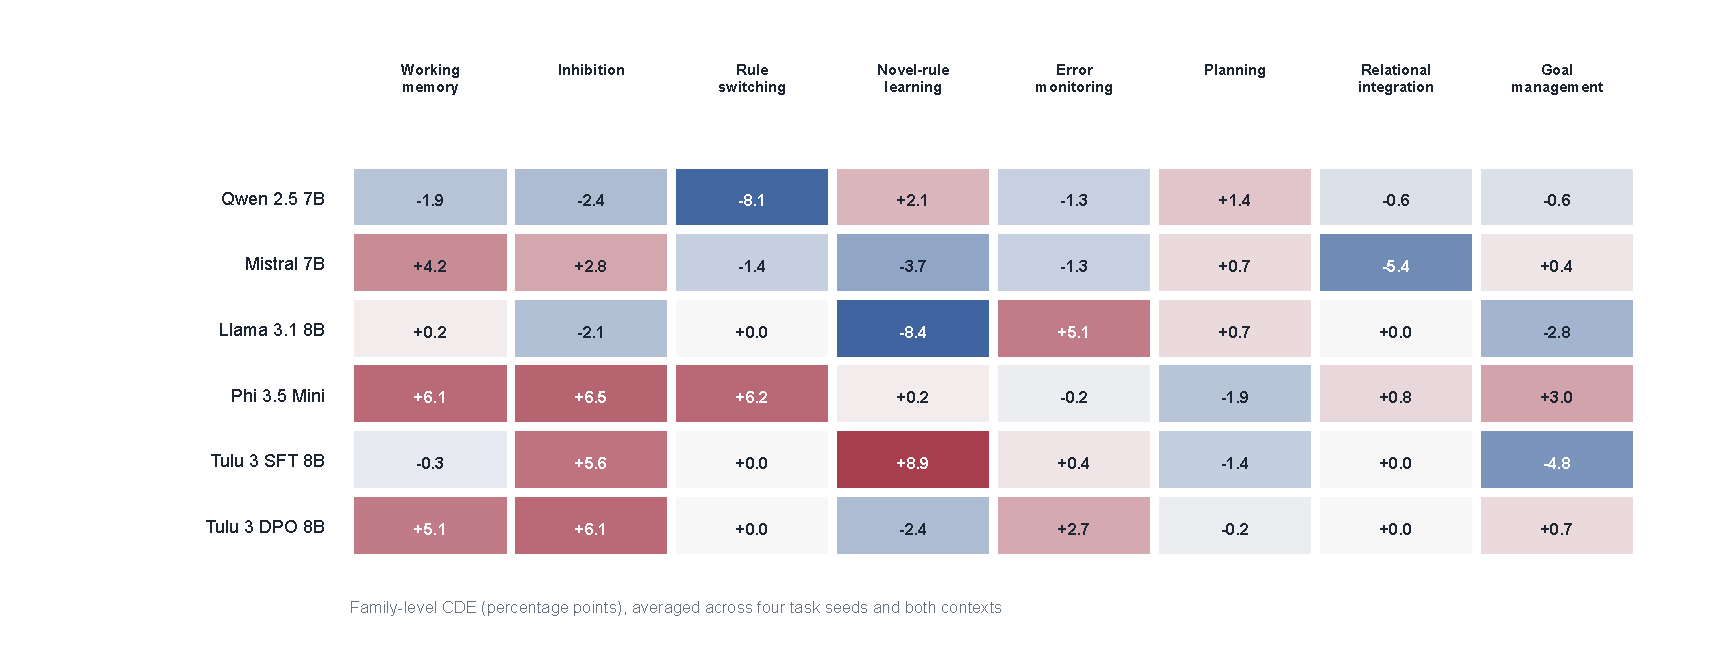
\includegraphics[width=0.96\textwidth]{figures/family_cde_heatmap.pdf}
\Description{Heat map of conditional doubt effects for six checkpoints across
eight task families and two task contexts. Colors range from negative effects
in blue to positive effects in red.}
\caption{CDE by checkpoint and task family, averaged across four task sets and
both contexts. The same prompt component can help one family and harm another
within a checkpoint.}
\label{fig:family-cde}
\end{figure*}

Family means span approximately $-8.4\pp$ to $+8.9\pp$. Examples include Qwen
on rule switching ($-8.1\pp$) versus novel-rule learning ($+2.1\pp$), Llama on
error monitoring ($+5.1\pp$) versus novel-rule learning ($-8.4\pp$), and
Tulu-SFT on novel-rule learning ($+8.9\pp$) versus goal management
($-4.8\pp$). Twenty-one nonzero checkpoint--family effects retain the same
direction in all four task sets. These decompositions are descriptive; CDE
pooled over families is the primary endpoint.

\begin{table}[t]
\centering\scriptsize
\caption{CDE by generated difficulty (percentage points), averaged over four task seeds and both contexts.}
\label{tab:difficulty-cde}
\begin{tabular}{@{}lrrr@{}}
\toprule
Checkpoint & Easy & Medium & Hard \\
\midrule
Qwen 2.5 7B & -1.25 & -2.05 & -0.55 \\
Mistral 7B & -1.48 & -0.80 & +2.23 \\
Llama 3.1 8B & -1.33 & -0.45 & -1.05 \\
Phi 3.5 Mini & +0.82 & +3.40 & +4.49 \\
Tulu 3 SFT 8B & -0.39 & +1.62 & +2.73 \\
Tulu 3 DPO 8B & +1.46 & +0.96 & +2.70 \\
\bottomrule
\end{tabular}
\end{table}


Difficulty moderates some checkpoints but not in a common monotonic direction.
For example, Phi rises from $+0.82\pp$ on easy tasks to $+4.49\pp$ on hard
tasks, while Qwen and Mistral do not show the same pattern.

\subsection{Within-Lineage Post-Training Comparison}

Table~\ref{tab:tulu} compares the two checkpoints that share the Tulu
post-training lineage.

\begin{table}[H]
\centering\small
\begin{tabular}{@{}lrrr@{}}
\toprule
Endpoint & Tulu SFT & Tulu DPO & DPO $-$ SFT \\
\midrule
Neutral accuracy & 13.52 & 16.30 & +2.78 \\
Checking gain & -0.12 & +1.79 & +1.91 \\
Overall CDE & +1.04 & +1.51 & +0.47 \\
CDE, minimal & +1.13 & +2.52 & +1.39 \\
CDE, reasoning requested & +0.95 & +0.50 & -0.45 \\
Context modulation & -0.17 & -2.02 & -1.84 \\
Concision effect & +1.32 & -3.74 & -5.06 \\
\bottomrule
\end{tabular}
\caption{Within-lineage comparison in percentage points. This single
foundation lineage does not identify a general effect of SFT or DPO.}
\label{tab:tulu}
\end{table}

DPO increases neutral accuracy and minimal-context CDE relative to SFT, while
slightly decreasing reasoning-requested CDE. The evidence supports the narrow
claim that these two post-training checkpoints have different prompt-response
profiles, not that DPO generally increases or decreases susceptibility to
self-doubt wording.

\section{Surface Robustness and Output-Format Effects}

\subsection{Answer-Preserving Surface Forms}

For every task type, ten latent tasks are selected with a 4/4/2
easy--medium--hard allocation. Each is evaluated in its canonical form and in
two answer-preserving forms: a sectioned structured form and a short
scenario-framed form. The same latent task and gold answer are used across all
three renderings. Figure~\ref{fig:surface} visualizes the changes across
renderings, and Table~\ref{tab:surface-cde} reports the corresponding exact
CDEs.

\begin{figure*}[t]
\centering
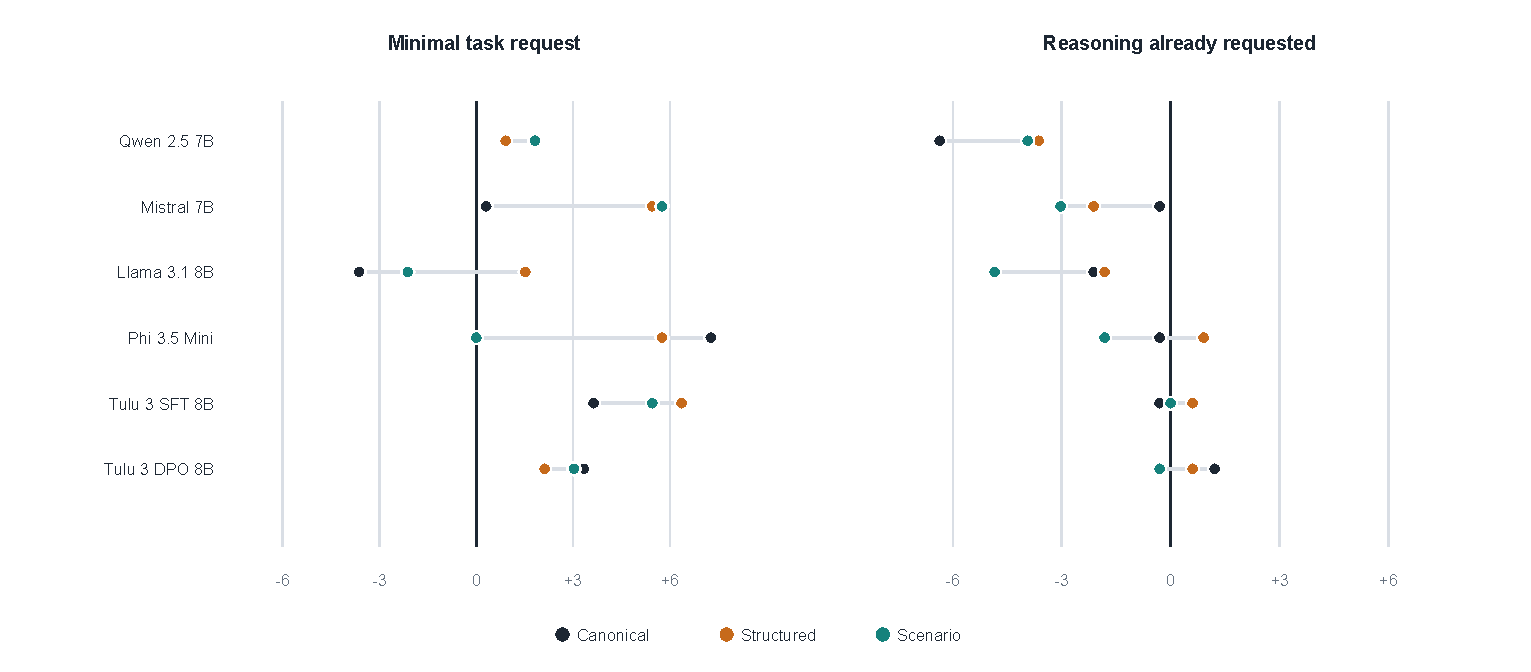
\includegraphics[width=0.94\textwidth]{figures/surface_cde_robustness.pdf}
\Description{Point plots comparing conditional doubt effects for canonical,
structured, and scenario renderings in minimal and reasoning-requested
contexts for six checkpoints.}
\caption{CDE on 330 paired latent tasks under canonical, structured, and
scenario renderings. Exact effect sizes move under answer-preserving wording,
especially for effects near zero.}
\label{fig:surface}
\end{figure*}

\begin{table}[t]
\centering\scriptsize
\caption{Surface-form CDE in percentage points on the same 330 latent tasks.}
\label{tab:surface-cde}
\begin{tabular}{@{}llrrr@{}}
\toprule
Checkpoint & Context & Canonical & Structured & Scenario \\
\midrule
Qwen 2.5 7B & Minimal & +0.91 & +0.91 & +1.82 \\
Qwen 2.5 7B & Reasoning & -6.36 & -3.64 & -3.94 \\
\addlinespace[1.5pt]
Mistral 7B & Minimal & +0.30 & +5.45 & +5.76 \\
Mistral 7B & Reasoning & -0.30 & -2.12 & -3.03 \\
\addlinespace[1.5pt]
Llama 3.1 8B & Minimal & -3.64 & +1.52 & -2.12 \\
Llama 3.1 8B & Reasoning & -2.12 & -1.82 & -4.85 \\
\addlinespace[1.5pt]
Phi 3.5 Mini & Minimal & +7.27 & +5.76 & +0.00 \\
Phi 3.5 Mini & Reasoning & -0.30 & +0.91 & -1.82 \\
\addlinespace[1.5pt]
Tulu 3 SFT 8B & Minimal & +3.64 & +6.36 & +5.45 \\
Tulu 3 SFT 8B & Reasoning & -0.30 & +0.61 & +0.00 \\
\addlinespace[1.5pt]
Tulu 3 DPO 8B & Minimal & +3.33 & +2.12 & +3.03 \\
Tulu 3 DPO 8B & Reasoning & +1.21 & +0.61 & -0.30 \\
\bottomrule
\end{tabular}
\end{table}


Across the 60 checkpoint--condition--context cells, mean three-way correctness
agreement is 81.3\%. The median absolute CDE shift from the canonical form is
$1.52\pp$. Seven of the 12 checkpoint--context CDE signs remain unchanged
across all three forms. Qwen and Mistral preserve their minimal-positive and
reasoning-negative patterns; several smaller effects cross zero. The robust
conclusion is therefore coarse heterogeneity rather than invariance of an
exact numerical effect.

\subsection{Concision as an Output-Format Intervention}

Figure~\ref{fig:concision} compares the change in accuracy with the change in
generated length when concision is added to the checking instruction.

\begin{figure*}[t]
\centering
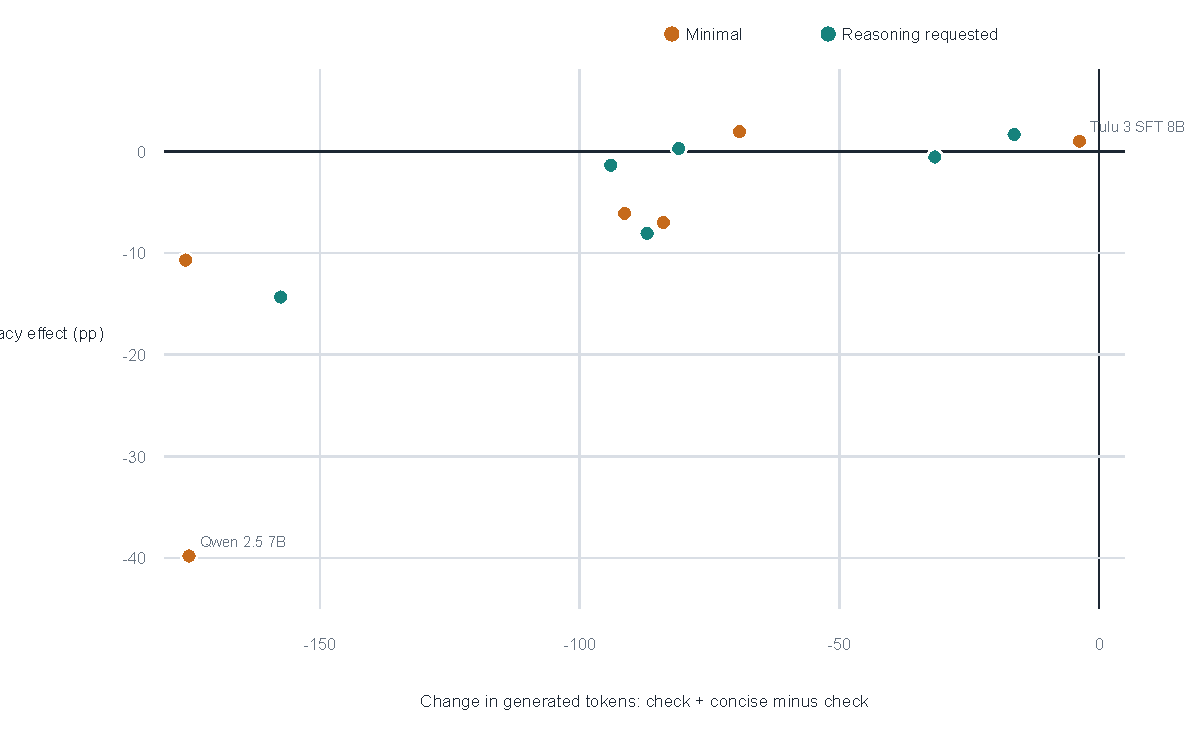
\includegraphics[width=0.84\textwidth]{figures/concision_accuracy_token_tradeoff.pdf}
\Description{Scatter plot of the change in exact accuracy against the change
in generated tokens when concise output is added to a checking instruction,
shown for six checkpoints in two task contexts.}
\caption{Change in exact accuracy and generated tokens when concise output is
required in addition to checking. Output length is an observable behavior, not
a measure of hidden computation.}
\label{fig:concision}
\end{figure*}

Across the 12 checkpoint--context cells, checking plus concision changes
accuracy by a median $-3.74\pp$ and generated length by a median $-85.4$
tokens relative to checking alone. The relationship is not uniform: some
Mistral and Tulu-SFT cells become slightly more accurate, whereas Qwen under a
minimal request loses approximately 40 accuracy points while generating about
175 fewer tokens. This control demonstrates that an apparently simple output
constraint can change both format and correctness.

\end{document}
